\documentclass[11pt,reqno]{amsart}
\usepackage{amsmath,amssymb,amsthm}
\usepackage{mathptmx}
\usepackage[scaled=0.90]{helvet}
\usepackage{courier}
\usepackage[T1]{fontenc}
\usepackage{enumitem}
\usepackage[hidelinks]{hyperref}
\pagestyle{plain}

\setlength{\oddsidemargin}{0cm}
\setlength{\evensidemargin}{0cm}
\setlength{\topmargin}{0in}
\setlength{\headheight}{0pt}
\setlength{\headsep}{0pt}
\setlength{\footskip}{.3in}
\setlength{\textheight}{9.2in}
\setlength{\textwidth}{6.5in}
\setlength{\parindent}{0pt}
\setlist[enumerate,1]{leftmargin=*,itemsep=1.1em}
\setlist[enumerate,2]{label=(\alph*),leftmargin=1.7em,itemsep=.45em,topsep=.4em}

\newcommand{\C}{\mathbb{C}}
\newcommand{\R}{\mathbb{R}}

\title{Problem Set 5: Solutions \\ MATH 411: Honors Complex Variables, Fall 2026}
\date{}

\usepackage[most]{tcolorbox}
\definecolor{solblue}{RGB}{232,243,252}
\definecolor{solframe}{RGB}{120,170,215}
\newenvironment{solution}
  {\par\smallskip\begin{tcolorbox}[breakable,enhanced,colback=solblue,colframe=solframe,
   boxrule=0.5pt,arc=2pt,left=6pt,right=6pt,top=4pt,bottom=4pt]\setlength{\abovedisplayskip}{7pt}\setlength{\belowdisplayskip}{7pt}\noindent\textbf{Solution.}}
  {\hfill$\square$\end{tcolorbox}\par\medskip}
\usepackage{needspace}
\widowpenalty=10000
\clubpenalty=10000
\raggedbottom


\DeclareMathOperator*{\Res}{Res}
% Earlier solutions (in Old Homework/Homework), indexed by the present numbering:
% 1, 3(a), 5, 6, 8--11: Homework5_Fall2021.tex, problems 5, 6(a), 8,
% 9--10, 11, 7, 12, 2. The real-integral proofs also appear in
% hwk4_solutions.tex (2020), problems 1--6.
% 3(b): corrected local expansion, as noted in HW5-draft/hw-05.tex.
% 13(a): Homework6_Fall2021solutions.tex, problem 2.
% 14: handwritten Homework 6 Solutions.pdf (2021), pp. 1--2.
% Contours are schematic. Arrowheads indicate the direction of integration.
\usepackage{tikz}
\usetikzlibrary{arrows.meta,decorations.markings}
\definecolor{contourink}{RGB}{25,72,106}
\tikzset{
  contour diagram/.style={x=0.82cm,y=0.82cm,font=\footnotesize,
    line cap=round,line join=round},
  complex axis/.style={gray!65,thin,-{Stealth[length=3pt]}},
  oriented/.style={draw=contourink,line width=1pt,
    decoration={markings,mark=at position #1 with
    {\arrow{Stealth[length=4.8pt,width=4.3pt]}}},postaction={decorate}},
  oriented/.default=.54,
  axis label/.style={font=\scriptsize,text=black!65,inner sep=1pt}}
\newcommand{\withcontour}[2]{\par\smallskip\noindent
  \begin{minipage}[c]{.675\linewidth}#1\end{minipage}\hfill
  \begin{minipage}[c]{.315\linewidth}\centering #2\end{minipage}\par\smallskip}
\newcommand{\circleaxes}{%
  \draw[complex axis] (-1.48,0)--(1.65,0) node[right,axis label] {$\Re$};
  \draw[complex axis] (0,-1.28)--(0,1.49) node[above,axis label] {$\Im$};
  \node[below left,axis label] at (0,0) {$0$};}
\newcommand{\onecircle}[1]{\begin{tikzpicture}[contour diagram]
  \circleaxes
  \draw[oriented=.14] (1,0) arc[start angle=0,end angle=360,radius=1];
  \node[below right,inner sep=1pt] at (1,0) {$#1$};
\end{tikzpicture}}
\newcommand{\twocircles}[2]{\begin{tikzpicture}[contour diagram]
  \circleaxes
  \draw[oriented=.14] (1.08,0) arc[start angle=0,end angle=360,radius=1.08];
  \draw[oriented=.37] (.47,0) arc[start angle=0,end angle=360,radius=.47];
  \node[below right,inner sep=1pt] at (1.08,0) {$#2$};
  \node[above right,inner sep=1pt] at (.47,0) {$#1$};
\end{tikzpicture}}
\newcommand{\clockwiserectangle}{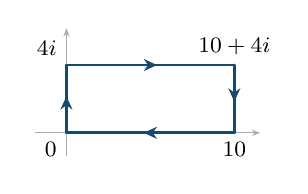
\begin{tikzpicture}[contour diagram]
  \draw[complex axis] (-.48,0)--(3.0,0);
  \draw[complex axis] (0,-.35)--(0,1.62);
  \draw[oriented] (0,0)--(0,1.05);
  \draw[oriented] (0,1.05)--(2.6,1.05);
  \draw[oriented] (2.6,1.05)--(2.6,0);
  \draw[oriented] (2.6,0)--(0,0);
  \node[below left] at (0,0) {$0$}; \node[below] at (2.6,0) {$10$};
  \node[above left] at (0,1.05) {$4i$};
  \node[above] at (2.6,1.05) {$10+4i$};
\end{tikzpicture}}
\newcommand{\uppersemicircle}{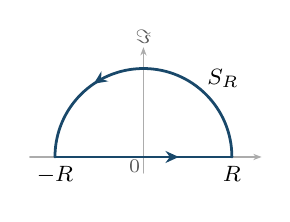
\begin{tikzpicture}[contour diagram]
  \draw[complex axis] (-1.76,0)--(1.83,0);
  \draw[complex axis] (0,-.25)--(0,1.7) node[above,axis label] {$\Im$};
  \draw[oriented=.7] (-1.37,0)--(1.37,0);
  \draw[oriented=.69] (1.37,0) arc[start angle=0,end angle=180,radius=1.37];
  \node[below] at (-1.37,0) {$-R$}; \node[below] at (1.37,0) {$R$};
  \node[below left,axis label] at (0,0) {$0$};
  \node[above right,inner sep=1pt] at (.94,1.02) {$S_R$};
\end{tikzpicture}}
\newcommand{\indentedsemicircle}{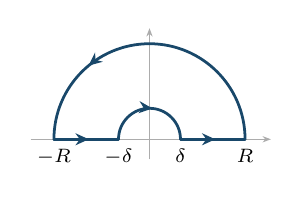
\begin{tikzpicture}[contour diagram]
  \draw[complex axis] (-1.83,0)--(1.88,0);
  \draw[complex axis] (0,-.3)--(0,1.72);
  \draw[oriented] (-1.48,0)--(-.48,0);
  \draw[oriented=.53] (-.48,0) arc[start angle=180,end angle=0,radius=.48];
  \draw[oriented] (.48,0)--(1.48,0);
  \draw[oriented=.72] (1.48,0) arc[start angle=0,end angle=180,radius=1.48];
  \foreach \x/\lab in {-1.48/{-R},-.48/{-\delta},.48/{\delta},1.48/{R}}
    \node[below,font=\scriptsize] at (\x,0) {$\lab$};
\end{tikzpicture}}
\newcommand{\gaussiancontour}{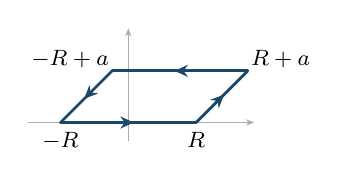
\begin{tikzpicture}[contour diagram]
  \draw[complex axis] (-1.55,0)--(1.95,0);
  \draw[complex axis] (0,-.28)--(0,1.46);
  \coordinate (a) at (-1.05,0); \coordinate (b) at (1.05,0);
  \coordinate (c) at (1.85,.8); \coordinate (d) at (-.25,.8);
  \draw[oriented] (a)--(b); \draw[oriented] (b)--(c);
  \draw[oriented] (c)--(d); \draw[oriented] (d)--(a);
  \node[below] at (a) {$-R$}; \node[below] at (b) {$R$};
  \node[above right,inner sep=1pt] at (c) {$R+a$};
  \node[above left,inner sep=1pt] at (d) {$-R+a$};
\end{tikzpicture}}
\newcommand{\samplepath}{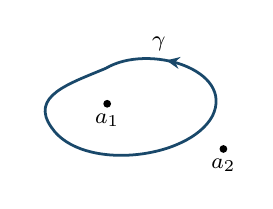
\begin{tikzpicture}[contour diagram]
  \draw[oriented=.2] (1.2,0) .. controls (1.55,.72) and (.21,1.13) .. (-.45,.74)
    .. controls (-1.02,.50) and (-1.64,.31) .. (-1.29,-.18)
    .. controls (-.83,-.86) and (.83,-.68) .. (1.2,0);
  \node[above] at (.37,.86) {$\gamma$};
  \fill (-.43,.19) circle (1.4pt) node[below] {$a_1$};
  \fill (1.37,-.51) circle (1.4pt) node[below] {$a_2$};
\end{tikzpicture}\par{\scriptsize One possible path}}

\begin{document}
\maketitle
Unless stated otherwise, closed contours are oriented counterclockwise.
\begin{enumerate}
\item \textbf{Residues at the origin.}
Find the residue at $0$ of each of the following.
\[
\text{(a)}\quad \dfrac{2z+1}{z(z^3-5)}\qquad \text{(b)}\quad \dfrac{e^z}{z^4}\qquad \text{(c)}\quad \dfrac{e^z}{\sin z}
\]
Also find the residue at $z=1$ of
\[
 \frac{(z^3-1)(z+2)}{(z^4-1)^2}.
\]

\begin{solution}
(a) The pole is simple. Multiplying by $z$ and setting $z=0$ gives
$(2z+1)/(z^3-5)|_{z=0}=\boxed{-1/5}$.

\smallskip
(b) The coefficient of $z^{-1}$ in $e^z/z^4$ is the coefficient of
$z^3$ in $e^z$, namely $\boxed{1/3!}$.

\smallskip
(c) Since $\sin z$ has a simple zero at $0$, the residue is
$e^0/\cos 0=\boxed{1}$.

\smallskip
At $z=1$, cancel one factor of $z-1$. The remaining pole is simple, with residue
\[
 \left.\frac{(z^2+z+1)(z+2)}{(z^3+z^2+z+1)^2}\right|_{z=1}
 =\boxed{\frac{9}{16}}.
\]
\end{solution}

\item \textbf{Contour integrals by residues.}
\withcontour{%
Locate and classify the isolated singularities of the integrand, then
evaluate
\[
 \int_{|z|=r}\frac{e^z-1}{z^3(z-2)}\,dz
 \qquad\text{for }r=1\text{ and }r=3.
\]%
}{\twocircles{1}{3}}


\begin{solution}
At $0$ the numerator has a simple zero, so there is a pole of order two.
Multiplying the first terms of the two series gives
\[
 \frac{e^z-1}{z^3(z-2)}
 =-\frac{1}{2z^2}\left(1+\frac z2+O(z^2)\right)
                   \left(1+\frac z2+O(z^2)\right)
 =-\frac{1}{2z^2}-\frac{1}{2z}+O(1).
\]
At $2$ there is a simple pole with residue $(e^2-1)/8$. These are the only
finite singularities. The circle of radius $1$ encloses just $0$, while
the circle of radius $3$ encloses both poles. The residue theorem gives
\[
 r=1:\quad 2\pi i\left(-\frac12\right)=\boxed{-\pi i},
 \qquad
 r=3:\quad 2\pi i\left(-\frac12+\frac{e^2-1}{8}\right)
   =\boxed{\frac{\pi i}{4}(e^2-5)}.
\]
\end{solution}


\newpage
\item \textbf{Contour integrals by residues.}
\begin{enumerate}
\item \withcontour{%
Evaluate
\[
 \int_C\frac{dz}{z^2-3z+5},
\]
where $C$ is the boundary of the rectangle with vertices
$0,\ 10,\ 10+4i,\ 4i$, oriented \emph{clockwise}.%
}{\clockwiserectangle}
\item \withcontour{%
Evaluate
\[
 \int_C\frac{1+z}{1-\sin z}\,dz,
\]
where $C$ is the circle $|z|=8$. \emph{Hint:} First find all complex
solutions of $\sin z=1$ and determine the order of each zero of
$1-\sin z$.%
}{\onecircle{8}}
\end{enumerate}

\begin{solution}
(a) The quadratic polynomial $p(z)=z^2-3z+5$ has roots
$z_1=(3+i\sqrt{11})/2$ and $z_2=(3-i\sqrt{11})/2$. Only the first is
within the rectangle. The residue of $1/p(z)$ at $z_1$ is
$1/(z_1-z_2)=1/(i\sqrt{11})$. The clockwise orientation gives
\[
 \int_C\frac{dz}{p(z)}=-2\pi i\,\frac{1}{i\sqrt{11}}
 =\boxed{-\frac{2\pi}{\sqrt{11}}}.
\]

(b) Put $u=e^{iz}$. Then $\sin z=1$ gives $u-u^{-1}=2i$, or
$(u-i)^2=0$. Thus $e^{iz}=i$, so $z=c_k=\pi/2+2\pi k$ for $k\in\mathbb Z$.
Writing $h=z-c_k$, we have $1-\sin z=1-\cos h=h^2/2+O(h^4)$.
Each zero is double, and the expansion at that zero is
\[
 \frac{1+z}{1-\sin z}
  =(1+c_k+h)\left(\frac{2}{h^2}+O(1)\right)
  =\frac{2(1+c_k)}{h^2}+\frac2h+O(1).
\]
The three poles inside $|z|=8$ are $-3\pi/2$, $\pi/2$ and $5\pi/2$.
Each has residue $2$, so the integral is $2\pi i(2+2+2)=\boxed{12\pi i}$.
\end{solution}

\newpage
\item \textbf{A trigonometric integral.}
\emph{Reminder for Questions 4 and 5.}
As $t$ runs from $0$ to $2\pi$, the point $z=e^{it}$ traverses the unit
circle once counterclockwise. Since $e^{-it}=z^{-1}$ and $dz=iz\,dt$,
any rational function $R(\cos t,\sin t)$ whose denominator is nonzero
along the circle satisfies
\[
 \int_0^{2\pi} R(\cos t,\sin t)\,dt
 =\oint_{|z|=1}
 R\!\left(\frac{z+z^{-1}}{2},\frac{z-z^{-1}}{2i}\right)
 \frac{dz}{iz}.
\]
The residue theorem evaluates the right side using the poles inside $|z|<1$.

\smallskip
\withcontour{%
Use the substitution $z=e^{it}$ and the residue theorem to evaluate
\[
 \int_0^{2\pi}\frac{\cos(2t)}{5-4\cos t}\,dt.
\]
\emph{Hint.} Write $\cos(2t)=\operatorname{Re}(e^{2it})$.%
}{\onecircle{1}}


\begin{solution}
Let $J$ be the same integral with $e^{2it}$ in the numerator.
The required integral is $\operatorname{Re} J$. With $z=e^{it}$ we get
\[
 J=\frac1i\int_{|z|=1}\frac{z^2}{5z-2(z^2+1)}\,dz
   =-\frac{1}{2i}\int_{|z|=1}\frac{z^2}{(z-2)(z-1/2)}\,dz .
\]
Only $1/2$ lies inside the circle. Thus
$J=-\frac{2\pi i}{2i}\frac{(1/2)^2}{1/2-2}=\pi/6$.
Taking the real part gives $\boxed{\pi/6}$.
\end{solution}


\item \textbf{A trigonometric integral.}
\withcontour{%
Show that
\[
 \int_0^{2\pi}\frac{dt}{(5-3\sin t)^2}=\frac{5\pi}{32}.
\]%
}{\onecircle{1}}


\begin{solution}
Put $z=e^{it}$, so that $\sin t=(z-z^{-1})/(2i)$ and $dt=dz/(iz)$.
The integral becomes the unit-circle integral of
\[
 f(z)=\frac{4iz}{(-3z^2+10iz+3)^2}
     =\frac{4iz}{9(z-i/3)^2(z-3i)^2}.
\]
Only the double pole at $c=i/3$ lies in the circle. Write
$4iz=4i(z-c)-4/3$. The first term contributes $4i/[9(c-3i)^2]=-4i/64$
to the residue. For the second we need the linear coefficient of
$(z-3i)^{-2}$ at $c$, giving the contribution
$(-4/27)(-2)(c-3i)^{-3}=-i/64$. The integral is therefore
$2\pi i(-5i/64)=\boxed{5\pi/32}$.
\end{solution}

\newpage
\item \textbf{Rational integrals over the real line.}
\withcontour{%
\begin{enumerate}
\item Show that
\[
 \int_0^\infty\frac{x^2}{x^6+1}\,dx=\frac{\pi}{6}.
\]
\item For $a,b>0$, show that
\[
 \int_0^\infty\frac{dx}{(x^2+a^2)(x^2+b^2)}=\frac{\pi}{2ab(a+b)}.
\]
\end{enumerate}%
}{\uppersemicircle}


\begin{solution}
(a) Let $f(z)=z^2/(1+z^6)$. Since $f(-z)=f(z)$, the integral on the
whole real line is twice the one we want. Close the segment $[-R,R]$
by the upper semicircle $S_R$. For $R>1$ its contribution is bounded by
$\pi R^3/(R^6-1)\to0$. The upper poles are the three sixth roots of $-1$
at $e^{i\pi/6},i,e^{5i\pi/6}$. At each such point $c$ the residue is
$c^2/(6c^5)=1/(6c^3)$. In the indicated order the residues are
$-i/6,i/6,-i/6$. Thus the whole-line integral is $2\pi i(-i/6)=\pi/3$,
and the half-line integral is $\boxed{\pi/6}$.

\smallskip
(b) Use the same contour for $f(z)=1/[(z^2+a^2)(z^2+b^2)]$. For
$R>\max(a,b)$ the arc integral is bounded by
$\pi R/[(R^2-a^2)(R^2-b^2)]\to0$. If $a\ne b$, the upper poles $ia,ib$
are simple. Their residues are $1/[2ia(b^2-a^2)]$ and
$1/[2ib(a^2-b^2)]$, respectively. By evenness the desired integral is
\[
 \frac{\pi}{2(b^2-a^2)}\left(\frac1a-\frac1b\right)
 =\boxed{\frac{\pi}{2ab(a+b)}}.
\]
If $b=a$, the upper pole is double. Its residue is
$[(z+ia)^{-2}]'_{z=ia}=-2/(2ia)^3$. Multiplying by $\pi i$ gives
$\pi/(4a^3)$, precisely the same formula at $b=a$.
\end{solution}


\item \textbf{An improper integral.}
\withcontour{%
For $a>0$, use an upper-half-plane contour to evaluate
\[
 \int_{-\infty}^{\infty}\frac{\cos(ax)}{(x^2+4)^2}\,dx.
\]
Give an explicit bound for the integral of $e^{iaz}/(z^2+4)^2$
over the semicircular arc $|z|=R$, $\operatorname{Im}z\geq0$, for $R>2$.%
}{\uppersemicircle}


\begin{solution}
Set $F(z)=e^{iaz}/(z^2+4)^2$. On the upper semicircle $S_R$ we have
$|e^{iaz}|=e^{-a\operatorname{Im}z}\le1$ and $|z^2+4|\ge R^2-4$.
The length estimate gives the requested bound
\[
 \left|\int_{S_R}F(z)\,dz\right|\le
 \boxed{\frac{\pi R}{(R^2-4)^2}}\longrightarrow0 \qquad(R>2).
\]
Only the double pole $2i$ lies inside the contour. Its residue is
\[
 \left.\frac{d}{dz}\frac{e^{iaz}}{(z+2i)^2}\right|_{z=2i}
 =e^{-2a}\left(\frac{ia}{(4i)^2}-\frac{2}{(4i)^3}\right)
 =\frac{(2a+1)e^{-2a}}{32i}.
\]
The real-axis integral converges absolutely. Letting $R\to\infty$ and
taking real parts of $2\pi i$ times this residue gives
$\boxed{\pi(2a+1)e^{-2a}/16}$.
\end{solution}

\newpage
\item \textbf{A Fourier-type integral.}
\withcontour{%
For $a,b>0$ with $a\neq b$, show that
\[
 \int_{-\infty}^{\infty}\frac{\cos x}{(x^2+a^2)(x^2+b^2)}\,dx
 =\frac{\pi}{a^2-b^2}\left(\frac{e^{-b}}{b}-\frac{e^{-a}}{a}\right).
\]%
}{\uppersemicircle}


\begin{solution}
Let $f(z)=1/[(z^2+a^2)(z^2+b^2)]$. Since $f$ is even, the sine term
integrates to zero on $[-R,R]$. Thus we may compute the whole-line integral
of $f(x)e^{ix}$. Close in the upper half-plane, where $|e^{iz}|\le1$.
The arc estimate from 6(b) applies, and the real-axis integral converges
absolutely. The poles at $ia$ and $ib$ are simple. Writing
\[
 f(z)e^{iz}=\frac{1}{z-ia}\frac{e^{iz}}{(z+ia)(z^2+b^2)}
\]
gives the residue $e^{-a}/[2ia(b^2-a^2)]$ at $ia$. Interchanging
$a$ and $b$ gives $e^{-b}/[2ib(a^2-b^2)]$ at $ib$. Adding these and
multiplying by $2\pi i$, we obtain
\[
 \boxed{\frac{\pi}{a^2-b^2}\left(\frac{e^{-b}}b-\frac{e^{-a}}a\right)}.
\]
\end{solution}


\item \textbf{An integral with a logarithm.}
\withcontour{%
Show that
\[
 \int_0^\infty\frac{(\log x)^2}{1+x^2}\,dx=\frac{\pi^3}{8}.
\]
\emph{Hint:} Use a branch of $\log z$ on $\C$ minus the negative
imaginary axis, and integrate $(\log z)^2/(1+z^2)$ around the boundary
of the region $\{\delta\leq|z|\leq R,\ \operatorname{Im}z\geq0\}$
(Lang, \S VI.2, Exercise 14(a)). You may use
$\int_0^\infty dx/(1+x^2)=\pi/2$.%
}{\indentedsemicircle}


\begin{solution}
Choose the branch $\log z=\log|z|+i\theta$ with $-\pi/2<\theta<3\pi/2$.
For $0<\delta<1<R$ the only singularity inside the indicated contour is
the simple pole at $i$. The integral around the contour is therefore
\[
 2\pi i\,\frac{(\log i)^2}{2i}
 =2\pi i\,\frac{(i\pi/2)^2}{2i}=-\frac{\pi^3}{4}.
\]
On an upper semicircle of radius $s$, $|\log z|\le|\log s|+\pi$.
Hence the absolute value of the arc integral is at most
$\pi s(|\log s|+\pi)^2/|1-s^2|$, which tends to zero both as
$s=R\to\infty$ and as $s=\delta\downarrow0$.

For $x>0$, $\log(-x)=\log x+i\pi$. After putting $z=-x$ on the negative
real segment, the two straight pieces together give
\[
 \int_\delta^R\frac{(\log x+i\pi)^2+(\log x)^2}{1+x^2}\,dx .
\]
Taking real parts, then letting the radii tend to their limits, gives
$2I-\pi^2(\pi/2)=-\pi^3/4$, where $I$ is the required integral.
Thus $\boxed{I=\pi^3/8}$.
\end{solution}

\newpage
\item \textbf{The Gaussian integral via residues.}
\withcontour{%
Prove that
\[
 \int_{-\infty}^{\infty}e^{-x^2}\,dx=\sqrt{\pi}
\]
by integrating
\[
 f(z)=\frac{e^{-z^2}}{1+e^{-2az}},\qquad a=e^{\pi i/4}\sqrt{\pi},
\]
around the parallelogram with vertices $-R,\ R,\ R+a,\ -R+a$ and then
letting $R\to\infty$. \emph{Hint:} Check that $f(z)-f(z+a)=e^{-z^2}$.%
}{\gaussiancontour}


\begin{solution}
Since $a^2=i\pi$, we have $e^{-2a^2}=1$ and $e^{-a^2}=-1$. Thus
$f(z+a)=-e^{-2az}f(z)$, giving $f(z)-f(z+a)=e^{-z^2}$.
The denominator vanishes at the points $(k+1/2)a$, $k\in\mathbb Z$.
Only $a/2$ lies between the two horizontal edges. The pole is simple and
its residue is $e^{-a^2/4}/(2a)=1/(2i\sqrt\pi)$.

The opposite orientations on the two horizontal edges give their sum as
$\int_{-R}^R[f(x)-f(x+a)]\,dx=\int_{-R}^R e^{-x^2}\,dx$.
For the slanted sides put $c=\operatorname{Re}a=\operatorname{Im}a>0$.
At $z=\pm R+ta$, $0\le t\le1$, we have
\[
 |e^{-z^2}|\le e^{-R^2+2Rc},\qquad |e^{-2az}|=e^{\mp 2Rc}.
\]
The reverse triangle inequality bounds $|1+e^{-2az}|$ below by
$1-e^{-2Rc}$ on the right and $e^{2Rc}-1$ on the left. Since each side
has fixed length $|a|$, both side integrals tend to zero. The residue
theorem now gives $\int_{-\infty}^{\infty}e^{-x^2}\,dx
=2\pi i/(2i\sqrt\pi)=\boxed{\sqrt\pi}$.
\end{solution}


\item \textbf{Logarithmic derivatives.}
\begin{enumerate}
\item Show that the association $f\mapsto f'/f$ (for $f$ holomorphic
and nonvanishing) sends products to sums.
\item If $P(z)=(z-a_1)\cdots(z-a_n)$, where $a_1,\dots,a_n\in\C$ are
the roots of $P$ (listed with multiplicity), compute $P'/P$.
\item \withcontour{%
Let $\gamma$ be a closed path on which $P$ has no roots. Show
that
\[
 \frac{1}{2\pi i}\int_\gamma\frac{P'(z)}{P(z)}\,dz
 = W(\gamma,a_1)+\cdots+W(\gamma,a_n).
\]%
}{\samplepath}
\end{enumerate}

\begin{solution}
(a) From the product rule we have
$\displaystyle\frac{(fg)'}{fg}=\frac{f'g+fg'}{fg}=\frac{f'}f+\frac{g'}g$.

\smallskip
(b) Since $(z-a)'/(z-a)=1/(z-a)$, repeated application of (a) gives,
away from the roots,
\[
 \frac{P'(z)}{P(z)}=\sum_{j=1}^n\frac1{z-a_j}.
\]
A root of multiplicity $m$ occurs $m$ times in this sum.

(c) Integrate the finite sum over $\gamma$ and use the definition of the
winding number. This gives
\[
 \frac{1}{2\pi i}\int_\gamma\frac{P'(z)}{P(z)}\,dz
 =\sum_{j=1}^n\frac{1}{2\pi i}\int_\gamma\frac{dz}{z-a_j}
 =\sum_{j=1}^n W(\gamma,a_j).
\]
\end{solution}

\newpage
\item \textbf{The argument principle.}
\withcontour{%
For each $r>0$, let $C_r$ be the circle $|z|=r$. Consider
\[
 F(z)=\frac{(e^z-1)^2}{z^3(z-1)^2(z-3)}.
\]%
}{\twocircles{2}{7}}
\begin{enumerate}
\item Find all zeros and poles of $F$ in $|z|<7$, with their orders.
\item Use the argument principle to find the winding numbers $n_2$ and
$n_7$ of the image curves of $C_2$ and $C_7$ under $F$ about $0$.
What does $n_7-n_2$ count in the annulus $2<|z|<7$?
\end{enumerate}

\begin{solution}
(a) The zeros of $e^z-1$ are $2\pi i k$, $k\in\mathbb Z$, all simple
because $e^{2\pi i k}=1$. Squaring gives order two. At $0$, the
denominator has order three, leaving a simple pole. The complete list in
$|z|<7$ is therefore
\[
 \begin{array}{c|c}
 \text{zeros} & 2\pi i,\ -2\pi i\quad (\text{each of order }2)\\
 \text{poles} & 0\ (1),\quad 1\ (2),\quad 3\ (1).
 \end{array}
\]

(b) Neither circle meets a zero or pole. By the argument principle
the winding number of $F(C_r)$ is the number of zeros minus the number
of poles inside $C_r$, counted with orders. Hence
\[
 \boxed{n_2=0-(1+2)=-3},\qquad \boxed{n_7=4-(1+2+1)=0}.
\]
In general, $n_7-n_2$ counts the number of zeros minus the number of poles
of $F$ (with multiplicity) in the annulus $2<|z|<7$; here $n_7-n_2=3=4-1$,
coming from four zeros counted with multiplicity ($\pm2\pi i$, each double)
and one simple pole ($3$).
\end{solution}


\newpage
\item \textbf{Rouch\'e's theorem.}
\begin{enumerate}
\item How many zeros, counted with multiplicity, does
\[
 f(z)=z^5+5z^3+z^2+z+1
\]
have in the closed annulus $1\leq|z|\leq2$?

\item Let $a\in\C$ with $|a|\leq2$. Show that
$P_a(z)=z^6-6z^2+az+1$ has no zeros on $|z|=1$ or $|z|=2$.
How many zeros, counted with multiplicity, lie in each of the regions
$|z|<1$, $1<|z|<2$, and $|z|>2$? Justify the counts using
Rouch\'e's theorem.
\item Use Rouch\'e's theorem to prove the Fundamental Theorem of Algebra:
every complex polynomial of degree $n\geq1$ has exactly $n$ zeros in
$\C$, counted with multiplicity. \emph{Hint.} Compare the polynomial
with its leading term on a sufficiently large circle.
\end{enumerate}

\begin{solution}
(a) First compare $f$ with $g(z)=5z^3$ on $|z|=2$. There
$|f-g|\le32+4+2+1=39<40=|g|$. Thus Rouch\'e gives three zeros of $f$, counted with multiplicity, in the disc of radius $2$. On $|z|=1$
the same comparison gives $|f-g|\le4<5=|g|$. Both inequalities are
strict, so neither boundary contains a zero. All three zeros in the larger
disc are already in the smaller one. The closed annulus contains
$\boxed{0}$ zeros.

\smallskip
(b) On $|z|=1$, compare $P_a$ with $-6z^2$. The remaining terms have
modulus at most $1+2+1=4<6$. On $|z|=2$, compare with $z^6$.
Now the remaining terms have modulus at most $24+4+1=29<64$.
Both comparisons exclude boundary zeros. Rouch\'e gives two zeros inside
the first circle and six inside the second. Since $P_a$ has degree six,
the requested counts, in order, are $\boxed{2,\ 4,\ 0}$.

\smallskip
(c) Write $P(z)=c_nz^n+\cdots+c_0$ with $c_n\ne0$.
Choose $R>\max\{1,(\sum_{j<n}|c_j|)/|c_n|\}$, where $j$ runs from $0$
to $n-1$. For every $|z|\ge R$,
\[
 |P(z)-c_nz^n|\le |z|^{n-1}\sum_{j<n}|c_j|<|c_nz^n|.
\]
Rouch\'e on $|z|=R$ gives exactly $n$ zeros inside, counted with
multiplicity. The same strict inequality excludes any further zeros for
$|z|\ge R$.
\end{solution}


\newpage
\item \textbf{Images of the unit disc.}
Let $f$ be nonconstant and holomorphic on an open set containing the
closed unit disc $\overline{D}=\{|z|\leq1\}$, and let $D=\{|z|<1\}$.
\begin{enumerate}
\item Suppose $|f(z)|=1$ whenever $|z|=1$. Show that $f(D)$ contains
the open unit disc.
\item Suppose instead that $|f(z)|\geq1$ whenever $|z|=1$, and that
$|f(z_0)|<1$ for some $z_0\in D$. Show that $f(D)$ contains the open
unit disc.
\end{enumerate}
\emph{Hint:} For $|w|<1$, compare the number of zeros of $f$ and of
$f-w$ in $D$.

\begin{solution}
Let $|w_0|<1$. We want a solution of $f(z)=w_0$ with $z\in D$.
In both parts it suffices to show that $f$ has a zero in $D$. Indeed,
on the unit circle $|w_0|<1\le|f(z)|$, so Rouch\'e's theorem gives
the same number of zeros in $D$ for $f-w_0$ and for $f$.

\smallskip
(a) As usual, take $f$ to be nonconstant on the component containing
$\overline D$. The maximum modulus principle gives $|f|<1$ in $D$.
If $f$ had no zero there, $1/f$ would be holomorphic in $D$, continuous
on $\overline D$, and of modulus $1$ on the boundary. The maximum
modulus principle applied to $1/f$ would give $|f|\ge1$ throughout $D$,
a contradiction. Thus $f$ has the required zero.

\smallskip
(b) Again suppose $f$ has no zero in $D$. Now $|1/f|\le1$ on the
boundary, hence throughout $D$. At $z_0$ we would have
$|1/f(z_0)|>1$. This contradiction proves the claim.

\smallskip
\emph{On the hypothesis in (a).} If the open set is disconnected,
nonconstancy on that set alone is insufficient. For example, take $f=1$
on $|z|<2$ and $f=0$ on $|z-4|<1$. Then $f(D)=\{1\}$.
\end{solution}

\item \textbf{The open mapping theorem.}
Let $U\subseteq\C$ be a bounded domain and let $f$ be continuous on
$\overline U$ and holomorphic and nonconstant on $U$.
\begin{enumerate}
\item Use the open mapping theorem and compactness to prove that
$\partial(f(U))\subseteq f(\partial U)$.
\item For $U=\{z:|z-1|<2\}$ and $f(z)=z^2$, show that the inclusion is strict.
\end{enumerate}

\begin{solution}
(a) Take $w\in\partial(f(U))$ and choose $z_j\in U$ with $f(z_j)\to w$.
Since $U$ is bounded, $\overline U$ is compact. A subsequence of $z_j$
converges to some $z\in\overline U$, and continuity gives $f(z)=w$.
The open mapping theorem says that $f(U)$ is open, so its boundary
points lie outside $f(U)$. Consequently $z\in\partial U$, proving
$\partial(f(U))\subseteq f(\partial U)$.

\smallskip
(b) The boundary point $-1$ and the interior point $1$ have the same
square. Thus $1=f(-1)\in f(\partial U)$, while $1=f(1)$ lies in the
open set $f(U)$. In particular $1\notin\partial(f(U))$, so the
inclusion is strict.
\end{solution}

\end{enumerate}
\end{document}
